\chap{Sich ändernde Farben}

\sect{Zeige Farben an}

Erstelle ein VPL Programm, das zwei verschiedene Farben oben auf dem Roboter
anzeigt, wenn der Vorwärts- oder der Rückwärts-Knopf gedrückt wird. Wenn die
Links- und Rechts-Knöpfe gedrückt werden, sollen unten am Roboter zwei andere
Farben angezeigt werden.

{\raggedleft \hfill Beispielprogramm \bu{colors.aesl}}

Wir brauchen vier Ereignis-Aktions-Paare, da es vier verschiedene
Ereignisse---das Drücken der vier Knöpfe---gibt. Mit jedem Ereignis ist eine Farbaktion verbunden. 
Beachte den Unterschiede der Aktions-Blöcke für die obere Farben (\blksm{action-colors-up}) und 
die untere Farben \blksm{action-colors-down}) des Roboters. Der erste Block ändert die Farben, die auf der Oberseite des Roboters liegen, während der zweite die Farben der Unterseite des Roboters ändert. Im Block für die unteren Lichter sind die Räder als schwarze Balken abgebildet.

Das fertige Programm ist im Bild~\ref{fig.colors} dargestellt.

Welche Farben werden angezeigt? In den ersten drei Ereignis-Aktions-Paaren ist
jeweils eine Grundfarbe alleine gewählt. Die weissen Quadrate für die anderen
beiden Farben sind jeweils ganz links. Diese drei Aktionen werden also reines
Rot, Blau oder Grün anzeigen. Beim letzten Ereignis-Aktions-Paar werden aber
zwei Farben gemischt: die weissen Quadrate sind bei Rot und Grün ganz rechts.
Es wird also Rot und Grün gemischt. Welche Farbe entsteht daraus?

Dieses Programm ist in der Abbildung \cref{fig.colors-a} gezeigt.

Welche Farben werden angezeigt? In den ersten drei Aktionen ist der Schieberegler jeweils einer Farbe ganz nach rechts verschoben, während die Schieberegler der anderen Farben ganz links liegen. Deshalb werden diese Farben nicht dazugemischt und reines Rot, Blau oder Grün erscheint.
Die Aktion, welche mit dem linken Knopf verbunden ist, mixt die Farben Rot und Grün, was Gelb ergiebt.
Im Hintergrund siehst du wie sich die Farben ändern je nach Position des Schiebereglers. Die Farbe des Hintergrundes zeigt an, in welcher Farbe Thymio leuchten wird.

Lass das Programm (Icon \blksm{run}) laufen und überprüfe, ob sich durch das Drücken der Knöpfe die Farben des Roboters ändern.
\Cref{fig.front}  zeigt Thymio auf der Oberseite rot leuchtend und \cref{fig.bottom} zeigt Thymio auf der Unterseite grün leuchtend.

\exercisebox{\thechapter.1}{
Spiele mit dem Farbbalken und finde heraus welche Farben du anzeigen kannst.
Wie kannst du orange mischen?}

\sect{Schalte die Lichter aus}

Lass uns nun das Programm so verändern, dass alle Lichter ausgehen, wenn der
mittlere Knopf berührt wird. Wir brauchen also zwei neue
Ereignis-Aktions-Paare. Eines um die oberen und ein zweites,
um die unteren Lichter aus zu schalten. Damit die Lichter ausgehen, müssen wir alle drei
Schieberegler nach ganz links verschieben \cref{fig.colors-b}. So wird keine Farbe angezeigt und die Lichter werden ausgeschaltet.

Das \emph{Ereignis} ist jetzt für beide der neuen Ereignis-Aktions-Paare \emph{dasselbe}--- das Drücken des mittleren Knopfes---aber die \emph{Aktionen} sind \emph{unterschiedlich}.---das Ausschalten der Oberlicher und das Ausschalten der Unterlichter.

Vergiss nicht das Icon \blksmpure{run} zudrücken, damit das Programm geladen wird. In Zukunft werden wir diese Erinnerung nicht mehr bringen. Du brauchst jedoch jedesmal diese Funktion, um ein Programm zum Laufen zu bringen. 

\vfill

%\importantbox[Mehrere Ereignis-Aktions-Paare]{
\importantbox{Mehrere Ereignis-Aktions-Paare
\begin{itemize}[noitemsep,nosep,leftmargin=*]
\item Wenn ein Programm ausgeführt wird, werden alle Ereignis-Aktions-Paare
gleichzeitig ausgeführt.
\item Man kann mehrere Ereignis-Aktions-Paare mit dem gleichen Ereignis
    konstruieren, solange sie verschiedene Aktionen haben.
\item Sind zwei Ereignis-Aktions-Paare gleich (gleiches Ereignis und gleiche
    Aktion), zeigt VPL eine Fehlermeldung an. (Feld 3 in \cref{fig.vplgui}).
Es ist nicht möglich ein Programm laufenzulassen solange Fehlermeldungen angezeigt werden.
\end{itemize}
}

\begin{figure}
    \centering
    \subfigure[Die Farben verändern sich, wenn ein Knopf berührt wird.]{
		\label{fig.colors-a}
		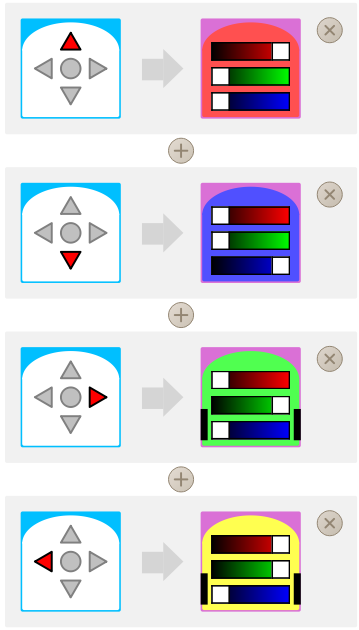
\includegraphics[width = 0.4\textwidth]{colors1}
	}
	\hspace{1.5cm}
    \subfigure[Lösche die Lichter mit dem mittleren Knopf.]{
		\label{fig.colors-b}
		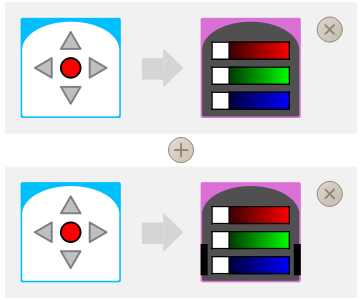
\includegraphics[width = 0.4\textwidth]{colors2}
	}
    \caption{Spiele mit den Lichter von Thymio}
    \label{fig.colors}
\end{figure}